\documentclass{beamer}
\setbeameroption{show notes}
\setbeamerfont{framesubtitle}{size=\normalfont\large}
\setbeamertemplate{footline}[frame number]
\setbeamertemplate{navigation symbols}{}


\usepackage[utf8]{inputenc}
\usepackage[T1]{fontenc}
% \usepackage[ngerman]{babel}

\usepackage{multicol}
\usepackage{prooftree}
\usepackage{bcprules}
\usepackage{scalefnt}
\usepackage{adjustbox}

\title{\\\emph{A Theory of Type Qualifiers}\\ 
\small{}Jeffrey S. Foster, Manuel Fähndrich, Alexander Aiken\\
PLDI 1999}
\author{Paper presentation by\\Georg Schmid and Samuel Grütter}
\date{May 20, 2015}

\usepackage{amssymb}
\usepackage{parskip}
\usepackage{listings}
\usepackage{graphicx}

\usepackage{todonotes}
\let\todox\todo
\renewcommand\todo[1]{\todox[inline]{#1}}

% Turnstile
\newcommand{\ts}{\,\vdash\,}

\begin{document}
\maketitle

\begin{frame}{Overview}
  \begin{itemize}
  \item Many languages support a range of \emph{type qualifiers} -- they enable a simple, yet useful form of subtyping.
      \todo{Give concrete examples of qualifiers}

  \item Authors present a framework for adding type qualifiers to $\lambda$-calculi.

  \item In particular, they show how to
    \begin{itemize}
    \item extend the typing rules, and
    \item support type inference --
    \item even in the polymorphic case.
    \end{itemize}
  \end{itemize}
\end{frame}


\defverbatim{\lstcduplicateprocs}{%
\begin{lstlisting}[language=C,frame=single,belowskip=- \medskipamount]
int *id1(int *x) { return x; }
const int *id2(const int *x) { return x; }
\end{lstlisting}}

\begin{frame}[fragile]{Motivation}
  \begin{itemize}
  \item Paper's presentation is closely tied to \textsc{const} qualifier in C

  \item[$\Rightarrow$] Use-case: Analyze C sources and infer additional \textsc{const} qualifiers

  \item<2->
    This rectifies one particular peculiarity of C's type system:
    % \vspace{1em}
    \lstcduplicateprocs
    $\rightarrow$ Inference of \textsc{const} qualifiers removes need for multiple versions of same procedure
    \todo{Replace with better example?}
  \end{itemize}
\end{frame}

\note[itemize]{%
  \item\emph{Q:} What does \textsc{const} in C mean?
  \todo{Will we show this to students? Why as notes?}}


\begin{frame}{Preliminaries}{Basic syntax / notation / definitions}
  \begin{itemize}
  \item type constructor, $\mathit{Typ}$ (paper\_typ.png), type environment
  \item framework allows mapping of source lang to lang with qualifiers; paper's source language (paper\_sourcelang)
  \item qualifiers, pos./neg. (paper\_negposqualifier), negation of a qualifier
  \item qualifier lattice (paper\_qualifierlattice\_\{def,sample\})
  \item intuition on qualifier lattice: losing ``information''/capabilites as we move up the lattice
  \end{itemize}
  \todo{Split into multiple slides and expand}
\end{frame}

\note[itemize]{%
  \item\emph{Q:} What is a two-point lattice?\\
  \item\emph{Q:} What is $\bot$ of this lattice? What is $\top$?\\
  \item\emph{Q:} ``Subset contradiction'' wrt.\ $\tau \subseteq \text{const}\ \tau$ (cf.\ dual notation as negative qualifier ``writable'' / consider \textsc{const} as ``read-only'' / rewrite as ``ConstInt'' $\geq$ ``NormalInt'' class hierarchy)\\
``WritableInt'' $\preceq$ ``NormalInt''}


\begin{frame}{Qualified types}
  \begin{itemize}
  \item $\mathit{QTyp}$ (paper\_qtyp), resulting concrete types wrt.\ sample lang
  \item subtyping rules (paper\_samplelang\_subtypingrules)
  \end{itemize}
\end{frame}


\begin{frame}{Qualifier annotations and assertions}
  \begin{itemize}
  \item purpose of annotations: support type inference -- problem: which type qualifier to choose for a given inferred type?
  \item ``qualifier annotations'' are added to the source language as a syntactic helper -- together with the resp.\ typing rule, qualifiers can only increase monotonically (``give up capabilities'')
  \item additionally, dual notion of ``qualifier assertions''
  \item source language extended (paper\_qualifierannass\_syntax), both enforce $e$'s top-level qualifier $Q_e$ to be upper-bounded by $l$, i.e.\ $Q_e \sqsubseteq l$ (-> Q)
  \item cf.\ typing rules (paper\_samplelang\_annasstyping)
  \end{itemize}
  \todo{Split into multiple slides and expand}
\end{frame}

\note[itemize]{%
  \item\emph{Q:} What's the difference between assertions and annotations? (Hint: Show typing rules)\\
  \item\emph{Q/Follow-up:} What's the difference between Q and l?}


\begin{frame}{Qualified type systems}
  \begin{center}\Large
  \begin{tabular}{l c r}
    $A \vdash e : \tau$ & $\Rightarrow$ & $A \vdash e : \rho$
  \end{tabular}
  \end{center}

  \vspace{1em}
  \large
  Extending the source language's type checking system with qualified types leads to a \emph{qualified type system}.
\end{frame}

\begin{frame}{Qualified type systems}{Typing rules of sample language (1)}
  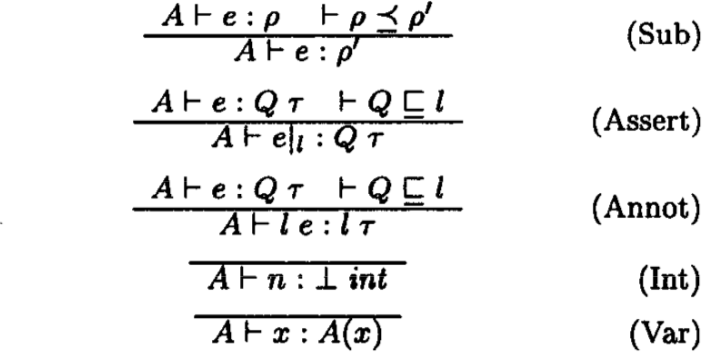
\includegraphics[scale=0.4]{paper_samplelang_typingrules1.png}
\end{frame}

\note[itemize]{%
  \item Discuss unrestricted type qualifier $Q$ in premises.
  \item Discuss how terminal expressions are assigned type qualifier $\bot$.}

\begin{frame}{Qualified type systems}{Typing rules of sample language (2)}
  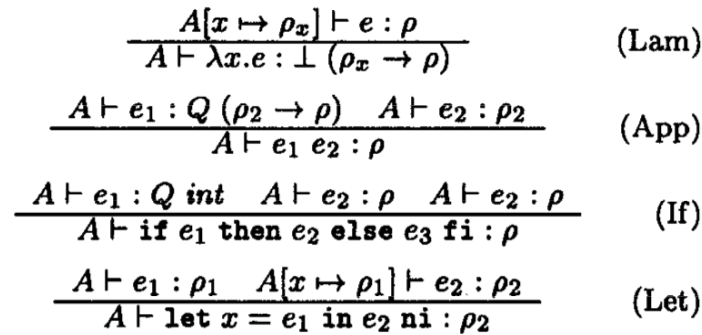
\includegraphics[scale=0.4]{paper_samplelang_typingrules2.png}
\end{frame}

\note[itemize]{\item\emph{Q:} Ad $(\text{App})$. What role do qualifiers on abstractions play in this paper?}


\begin{frame}{Qualified type systems}{Correspondence}
  \begin{itemize}
  \item type qualifiers should only refine type information,\\ but \emph{not} modify type structure
  \item[$\Rightarrow$] correspondence of the original and resp.\ qualified type system
  \item<2-> Helpers:\\
    \begin{description}
    \item[$\mathit{Typ} \rightarrow \mathit{QTyp}$:] $\text{strip}(\cdot)$ \ldots eliminates qualifiers \& annotations\\
      \visible<3->{\vspace{0.5em}\hspace{-4em}
        $\text{strip}(\,\overline{\bot(\text{const}\ \text{int} \to \text{nonzero}\ \text{int})}\,) =
         \overline{(\text{int} \to \text{int})}$
        }
    \item[$\mathit{QTyp} \rightarrow \mathit{Typ}$:] $\bot(\cdot)$ \ldots introduces $\bot$ qualifiers \& annotations\\
      \visible<4->{\vspace{0.5em}\hspace{-4em}
        $\bot(\,\overline{(\text{int} \to \text{int})}\,) =
          \overline{\bot(\bot\ \text{int} \to \bot\ \text{int})}$
        }
    \end{description}
  % \item[]<2->
  %   \begin{center}
  %   \vspace{1em}
  %   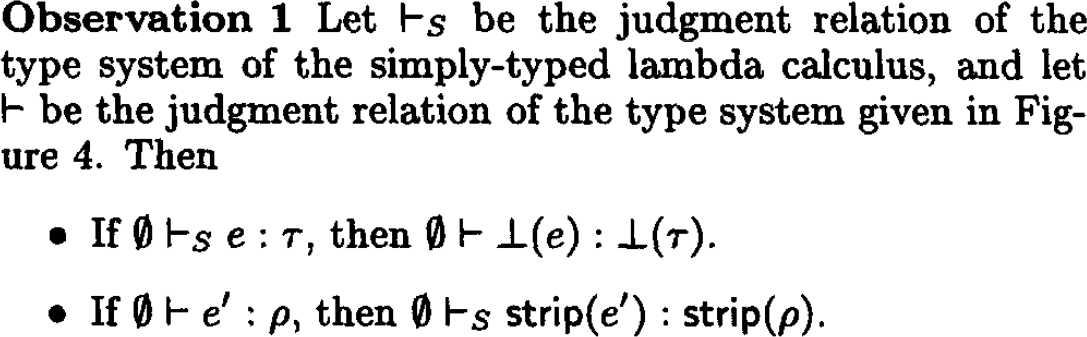
\includegraphics[scale=0.25]{paper_observation1.png}
  %   \end{center}
    \visible<4->{\todo{Verify that this is line with the paper's definition of $\bot(\cdot)$.}
      \todo{Improve readability.}}
  \end{itemize}
\end{frame}

% \note[itemize]{%
%   \item Discuss definition of $\bot(\cdot)$ and $\text{strip}(\cdot)$.}

\begin{frame}{Qualified type systems}{Correspondence (ctd.)}
  \begin{center}
  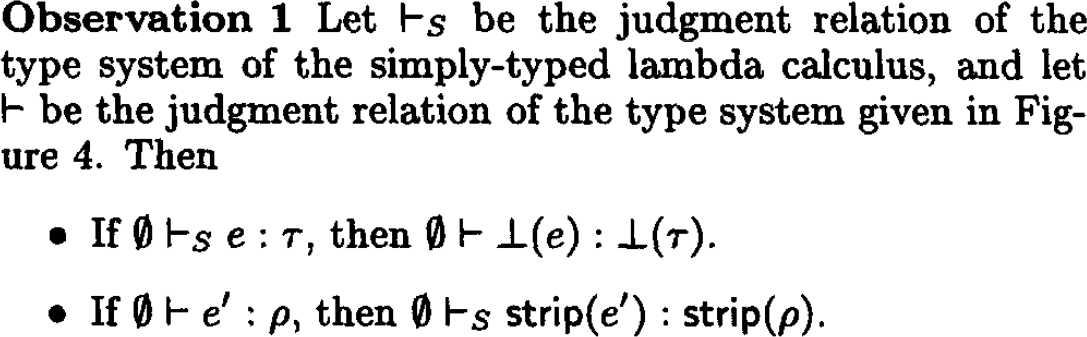
\includegraphics[scale=0.25]{paper_observation1.png}
  \end{center}
\end{frame}

\note[itemize]{%
  \item\emph{Q:} Ad $\bot(\cdot)$. Could we use $\top$ instead? Any other qualifier?\\\quad$\rightarrow$ Here, the choice of qualifier is unimportant.}


\begin{frame}{Qualifier semantics}
  \begin{itemize}
  \item Restrictions on usage of qualifiers can be expressed
    \begin{enumerate}[a)]
    % \item using qualifier assertions (injected during a preprocessing step of programs), or
    \item using qualifier assertions ($\rightarrow$ program transformation), or
    \item by modifying typing rules.
    \end{enumerate}
  \item Arbitrary modifications may render the type system unsound!
  \end{itemize}
\end{frame}

\begin{frame}{Qualifier semantics}{\textsc{const} example}
  \begin{itemize}
  \item Let's encode the semantics of a \textsc{const} qualifier!
  \item<2-> Only makes sense in presence of \emph{references}:
    \begin{center}
    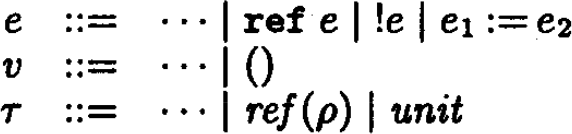
\includegraphics[scale=0.3]{paper_ref_syntax.png}
    \end{center}
  \end{itemize}
\end{frame}

\note{\emph{Q:} Why do they introduce unit / $()$? (Hint: Why only along with references?)}

\begin{frame}{Qualifier semantics}{\textsc{const} example (2)}
  \begin{itemize}
  \item A first attempt:
    \begin{center}
    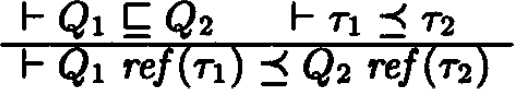
\includegraphics[scale=0.29]{paper_ref_unsound.png}
    \end{center}
  \item<2-> Unsound in the presence of subtyping!
    \begin{center}
    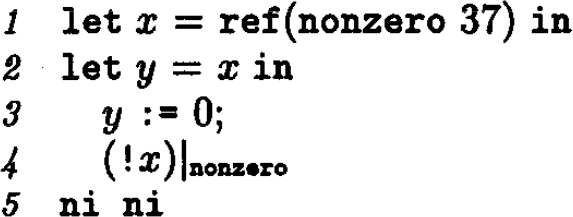
\includegraphics[scale=0.3]{paper_ref_unsoundsample.png}
    \end{center}
  \item<3->[$\Rightarrow$] Note that lines 3 and 4 type check, e.g.\
    \begin{minipage}[t]{0.3\textwidth}
    \begin{tabbing}
    \=\#3: \=$A[x, y \mapsto \bot\,\text{ref nonzero int}]\,\vdash y : \neg\text{nonzero int}$\quad \=\small(by $(\text{Sub})$)\\
    \>\#4: \>$A[x, y \mapsto \bot\,\text{ref nonzero int}]\,\vdash\ !x : \text{nonzero int}$ \>\small(unchanged)
    \end{tabbing}
    \end{minipage}
    \todo{Should introduce qualifier negation for this.}
  \end{itemize}
\end{frame}

\begin{frame}{Qualifier semantics}{\textsc{const} example (3)}
  \begin{itemize}
  \item Requiring refs' argument type to be invariant, fixes our problem.
    \begin{center}
    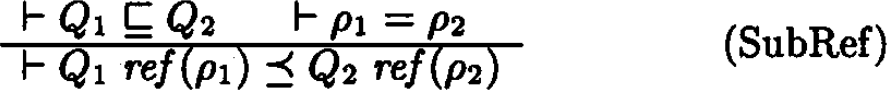
\includegraphics[scale=0.29]{paper_ref_sound.png}
    \end{center}
  \item<2-> Generally, subtyping rules of the form
    \begin{center}
    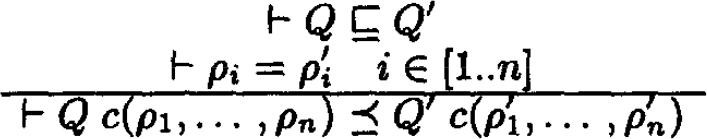
\includegraphics[scale=0.3]{paper_subtypingrule_general.png}
    \end{center}
    are sound.
  \end{itemize}
\end{frame}

\begin{frame}{Qualifier semantics}{\textsc{const} example (4)}
  \begin{itemize}
  \item How do we enforce the semantics of \textsc{const}?
  \item<2-> As mentioned before, there are two ways to encode such restrictions:
    \begin{enumerate}[a)]
    \item<2-> Program transformation:\\ Replace every assignment $e\,=\,e_1\!:=\!e_2$ by $e\!\mid_{\neg\text{const}}$.
    \item<3-> Modify the relevant typing rule(s):\\
      \begin{center}
      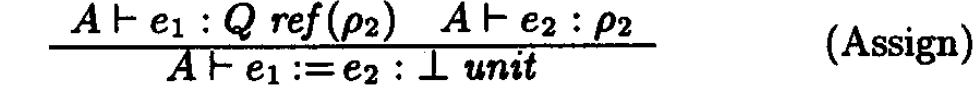
\includegraphics[scale=0.25]{paper_assign_original.png}\\
      \vspace{0.5em}{\Huge $\Downarrow$}\hspace{5.8em}\vspace{0.5em}\\
      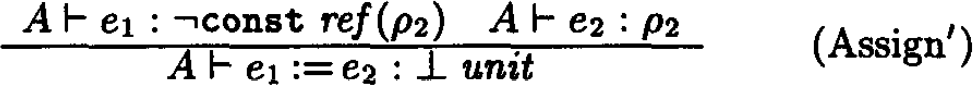
\includegraphics[scale=0.25]{paper_assign_adapted.png}
      \end{center}
    \end{enumerate}
  % \item<2-> Generally, subtyping rules of the form
  %   \begin{center}
  %   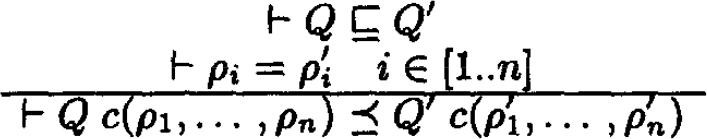
\includegraphics[scale=0.3]{paper_subtypingrule_general.png}
  %   \end{center}
  %   are sound.
  \end{itemize}
\end{frame}

%%%%%%%%%%%%%%%%%%%%%%% SECTION 3 & 4 %%%%%%%%%%%%%%%%%%%%%%%%%%%%%%%%%%%%%%%%%%


\begin{frame}{Type Inference and Qualifier Polymorphism}
Outline
\begin{enumerate}
\item Forget about qualifiers\\
Discuss type inference on simply typed lambda calculus
\item Add qualifiers
\item Add polymorphism
\end{enumerate}
\end{frame}

\begin{frame}{Step 1: Forget about qualifiers}

\infrule[Int]
{}
{A \ts n : int}

\infrule[Var]
{}
{A \ts x : A(x)}

\infrule[Lam]
{A[x \rightarrow \tau_1] \ts e : \tau_2}
{A \ts \lambda x . e : \tau_1 \rightarrow \tau_2}

\infrule[App]
{A \ts e_1 : \tau_2 \rightarrow \tau ~~~~ A \ts e_2 : \tau_2}
{A \ts e_1 e_2 : \tau}

\infrule[If]
{A \ts e_1 : int ~~~~ A \ts e_2 : \tau ~~~ A \ts e_3 : \tau}
{A \ts \text{\textbf{if }} e_1 \text{\textbf{ then }} e_2 \text{\textbf{ else }} e_3 \text{\textbf{ fi}} : \tau}

\infrule[Let]
{A \ts e_1 : \tau_1 ~~~~ A[x \rightarrow \tau_1] \ts e_2 : \tau_2}
{A \ts \text{\textbf{let }} x = e_1 \text{\textbf{ in }} e_2 \text{\textbf{ ni}} : \tau_2}

\end{frame}

\begin{frame}{The Problem}

Say we want to typecheck $\lambda x . <\text{some expression}>$.

Use

\infrule[Lam]
{A[x \rightarrow \tau_1] \ts e : \tau_2}
{A \ts \lambda x . e : \tau_1 \rightarrow \tau_2}

but what $\tau_1$ should we put into $A$?

\end{frame}

\begin{frame}{Solutions}

\begin{itemize}
\item Require users to write argument type\\
      $\lambda (x: \tau_1). e$ instead of $\lambda x . e$
\item Local type inference using \emph{expected types} (e.g. Scala)
      \texttt{List(1, 2, 3).map(x => x+1)}
\item Global type inference (e.g. ML)\\
  \textbf{let} $f = \lambda x . x + 1$ \textbf{in}\\
  $\dots$\\
  $myList.map(f)$\\
  $\dots$\\
  $otherList.map(f)$
\end{itemize}

\medskip

$\Longrightarrow$ Study \emph{Constraint-Based Typing}

\end{frame}

\begin{frame}{Constraint-Based Typing}

Approach:
\begin{enumerate}
\item Typecheck using the inference rules\\
      Whenever we don't know what type to choose, pick a fresh type variable $\alpha$ and record the constraints it has to satisfy
\item Unify the constraints
\end{enumerate}

\bigskip

Constraints = set of equality constraints:

%$C = \{ \tau_1 = \tau_1', ~ \tau_2 = \tau_2',~ \dots \}$

\includegraphics[scale=0.75]{paper_constraint_grammar.png}

\bigskip

New typing judgment:

%$A \ts e : \tau ; C$

\includegraphics[scale=0.75]{paper_constraint_judgment.png}

``In environment $A$, $e$ has type $\tau$ for all solutions of constraints $C$''

\end{frame}

\begin{frame}{Constraint-Based Typing Rules}

\infrule[Int]
{}
{A \ts n : int; \emptyset}

\infrule[Var]
{}
{A \ts x : A(x); \emptyset}

\infrule[Lam]
{\alpha \text{ fresh} ~~~~ A[x \rightarrow \alpha] \ts e : \tau_2 ; C}
{A \ts \lambda x . e : \alpha \rightarrow \tau_2 ; C}

\infrule[App]
{\alpha \text{ fresh} ~~~~ A \ts e_1 : \tau_1 ; C_1 ~~~~ A \ts e_2 : \tau_2 ; C_2}
{A \ts e_1 e_2 : \alpha ; C_1 \cup C_2 \cup \{ \tau_1 = (\tau_2 \rightarrow \alpha) \}}

\infrule[If]
{A \ts e_1 : \tau_1; C_1 ~~~~ A \ts e_2 : \tau_2; C_2 ~~~ A \ts e_3 : \tau_3; C_3}
{A \ts \text{\textbf{if }} e_1 \text{\textbf{ then }} e_2 \text{\textbf{ else }} e_3 \text{\textbf{ fi}} : \tau_2;\\
 C_1 \cup C_2 \cup C_3 \cup \{\tau_1 = int\} \cup \{\tau_2 = \tau_3\}}

\infrule[Let]
{A \ts e_1 : \tau_1; C_1 ~~~~ A[x \rightarrow \tau_1] \ts e_2 : \tau_2; C_2}
{A \ts \text{\textbf{let }} x = e_1 \text{\textbf{ in }} e_2 \text{\textbf{ ni}} : \tau_2; C_1 \cup C_2}

\end{frame}

\begin{frame}{Unification}

Solution to a set of constraints $C$ is a substitution


\includegraphics[scale=0.75]{paper_substitution_type.png}

mapping type variables to types containing no type variables,

such that all equalities in $SC$ hold.

\bigskip

Goal of unification: Given $C$, find $S$.

\end{frame}

\begin{frame}{Unification Algorithm}

\begin{small}

\textbf{def} unify$(C) = C$ \textbf{match} $\{$ \\
$~~$ \textbf{case} $\emptyset \Rightarrow$ identity   \textit{// empty substitution}\\
$~~$ \textbf{case} $c_1 \cup C_{rest} \Rightarrow c_1 $ \textbf{match} $\{$\\
$~~$ $~~$ \textbf{case} $((\tau_1 \rightarrow \tau_2) = (\tau_3 \rightarrow \tau_4)) \Rightarrow$ unify$(C_{rest} \cup \{\tau_1 = \tau_3\} \cup \{\tau_2 = \tau_4\})$\\
$~~$ $~~$ \textbf{case} $(\tau = \tau) \Rightarrow$ unify$(C_{rest})$\\
$~~$ $~~$ \textbf{case} $(\tau = \alpha)$ \textbf{if} $\alpha \notin FV(\tau) \Rightarrow$ unify$([\alpha \rightarrow \tau]C_{rest}) \circ [\alpha \rightarrow \tau]$\\
$~~$ $~~$ \textbf{case} $(\alpha = \tau)$ \textbf{if} $\alpha \notin FV(\tau) \Rightarrow$ unify$([\alpha \rightarrow \tau]C_{rest}) \circ [\alpha \rightarrow \tau]$\\
$~~$ $~~$ \textbf{case} \_ $\Rightarrow$ fail\\
$~~$ $\}$\\
$\}$

\end{small}

\end{frame}


\begin{frame}{Step 2: Add qualifiers}

\begin{tabular}{l | l}
Without qualifiers & With qualifiers \\
\hline

\includegraphics[scale=0.7]{paper_constraint_judgment.png} & 
\includegraphics[scale=0.55]{paper_constraint_judgment_qualifs.png}\\
\hline  
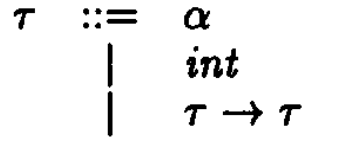
\includegraphics[scale=0.55]{paper_figure_1_tau.png} & 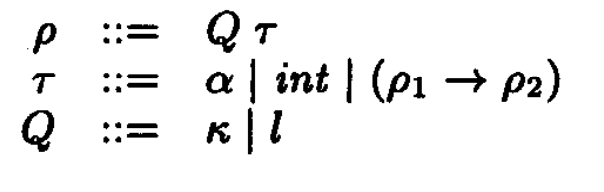
\includegraphics[scale=0.55]{paper_figure_3_no_label.png} \\
\hline

\includegraphics[scale=0.7]{paper_constraint_grammar.png} & 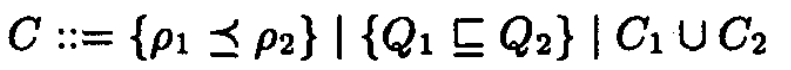
\includegraphics[scale=0.55]{paper_constraint_grammar_qualifs.png}\\
\hline
\end{tabular}

\bigskip
\pause

\textit{Q:} Why is there no $\rho_1 = \rho_2$ in the grammar for $C$?

\pause

\textit{A:} Because we can just use $\{\rho_1 \preceq \rho_2\} \cup \{\rho_2 \preceq \rho_1 \}$ instead.

\end{frame}

\begin{frame}{Constraint-Based Typing Rules With Qualifiers}

\infrule[Int]
{}
{A \ts n : int; \emptyset}

\infrule[Var]
{}
{A \ts x : A(x); \emptyset}

\infrule[Lam]
{\alpha \text{ fresh} ~~~~ \kappa \text{ fresh} ~~~~ A[x \rightarrow \kappa\alpha] \ts e : \rho_2 ; C}
{A \ts \lambda x . e : \kappa\alpha \rightarrow \tau_2 ; C}

\infrule[App]
{\alpha \text{ fresh} ~~~~ \kappa, \kappa' \text{ fresh} ~~~~ A \ts e_1 : \rho_1 ; C_1 ~~~~ A \ts e_2 : \rho_2 ; C_2}
{A \ts e_1 e_2 : \alpha ; C_1 \cup C_2 \cup \{ \rho_1 = \kappa(\rho_2 \rightarrow \kappa'\alpha) \}}

\infrule[If]
{\kappa \text{ fresh} ~~~~ A \ts e_1 : \rho_1; C_1 ~~~~ A \ts e_2 : \rho_2; C_2 ~~~ A \ts e_3 : \rho_3; C_3}
{A \ts \text{\textbf{if }} e_1 \text{\textbf{ then }} e_2 \text{\textbf{ else }} e_3 \text{\textbf{ fi}} : \rho_2;\\
 C_1 \cup C_2 \cup C_3 \cup \{\rho_1 = \kappa int\} \cup \{\rho_2 = \rho_3\}}

\infrule[Let]
{A \ts e_1 : \rho_1; C_1 ~~~~ A[x \rightarrow \rho_1] \ts e_2 : \rho_2; C_2}
{A \ts \text{\textbf{let }} x = e_1 \text{\textbf{ in }} e_2 \text{\textbf{ ni}} : \rho_2; C_1 \cup C_2}

\end{frame}

\begin{frame}{Question}

In an if-expression, what if the then-branch has type \texttt{const int} and the else-branch has type \texttt{int}: Can we still typecheck the expression?

(If) rule from previous slide:

\infrule[]
{\kappa \text{ fresh} ~~~~ A \ts e_1 : \rho_1; C_1 ~~~~ A \ts e_2 : \rho_2; C_2 ~~~ A \ts e_3 : \rho_3; C_3}
{A \ts \text{\textbf{if }} e_1 \text{\textbf{ then }} e_2 \text{\textbf{ else }} e_3 \text{\textbf{ fi}} : \rho_2;\\
 C_1 \cup C_2 \cup C_3 \cup \{\rho_1 = \kappa int\} \cup \{ \rho_2 = \rho_3\}}

\pause

A better version:

\infrule[]
{\alpha, \kappa, \kappa' \text{ fresh} ~~~~ A \ts e_1 : \rho_1; C_1 ~~~~ A \ts e_2 : \rho_2; C_2 ~~~ A \ts e_3 : \rho_3; C_3}
{A \ts \text{\textbf{if }} e_1 \text{\textbf{ then }} e_2 \text{\textbf{ else }} e_3 \text{\textbf{ fi}} : \kappa'\alpha;\\
 C_1 \cup C_2 \cup C_3 \cup \{\rho_1 = \kappa int\} \cup \{ \rho_2 \preceq \kappa'\alpha \} \cup \{ \rho_3 \preceq \kappa'\alpha \}}

\end{frame}

\begin{frame}{Unification Algorithm}

Reminder:\\ 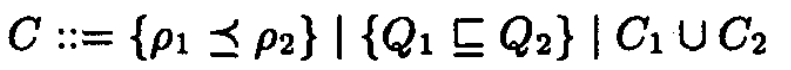
\includegraphics[scale=0.55]{paper_constraint_grammar_qualifs.png}

\bigskip

First phase: Repeat
\begin{itemize}
\item $\{(Q_1\tau_1 \rightarrow Q_2\tau_2) \preceq (Q_3\tau_3 \rightarrow Q_4\tau_4)\} \cup C_{rest}$ \\
$\Rightarrow C_{rest} \cup \{Q_3\tau_3 \preceq Q_1\tau_1\} \cup \{ Q_2\tau_2 \preceq Q_4\tau_4\})$
\item $\{Q\tau \preceq Q'\tau\} \cup C_{rest} ~~\Rightarrow~~ C_{rest} \cup \{ Q \sqsubseteq Q'\}$
\item $\{Q\tau \preceq Q'\alpha\} \cup C_{rest} ~~\Rightarrow~~ [\alpha \rightarrow \tau]C_{rest} \cup \{Q \sqsubseteq Q'\}$
\item $\{Q\alpha \preceq Q'\tau\} \cup C_{rest} ~~\Rightarrow~~ [\alpha \rightarrow \tau]C_{rest} \cup \{Q \sqsubseteq Q'\}$
\end{itemize}
until only lattice constrains are left.

Second phase:
\begin{itemize}
\item All constrains now are of the form $\kappa \sqsubseteq L$, $L \sqsubseteq \kappa$, or $L_1 \sqsubseteq L_2$.\\
Solve in linear time as described in [HR97].
\end{itemize}


\end{frame}


\begin{frame}{Test Page}%%%%%%%%%%%%%%%%

\begin{adjustbox}{width=0.3\textwidth}

Example: \textsc{invert-var}:

 \prooftree
	\prooftree
	   \dots
	\justifies
	    \Gamma \ts x : T' ~~
	\endprooftree
	\prooftree
	   \dots
	\justifies
	   \Gamma \ts T' <: T
	\endprooftree
\justifies
	\Gamma \ts x : T
\endprooftree
\end{adjustbox}

Example: \textsc{invert-var}:

 \prooftree
	\prooftree
	   \dots
	\justifies
	    \Gamma \ts x : T' ~~
	\endprooftree
	\prooftree
	   \dots
	\justifies
	   \Gamma \ts T' <: T
	\endprooftree
\justifies
	\Gamma \ts x : T
\endprooftree

\end{frame}


\end{document}